\section{Dataset}
Per condurre lo studio era necessario operare su un dataset che presentasse le caratteristiche tecniche adatte per l'analisi delle capacità di ogni modello nel riconoscere codice sicuro e vulnerabile.
Per perseguire questo obiettivo è stato utilizzato il dataset \enquote{\texttt{CodeXGLUE\_cc\_defect\_detection}}\cite{dataset}, il gold standard progettato specificatamente per la rilevazione di difetti per software AI-driven.
Sono stati selezionati snippet di codice sotto i 500 caratteri per evitare possibili scenari avversi allo studio, come l'uso completo della memoria che avrebbe portato ad un errore di Out of Memory (OOM), garantendo il successo degli attacchi e ridurre la possibilità di dispersione di questi ultimi così da assicurare l'analisi comportamentale del modello.
Il dataset ottenuto è quindi composto da 851 snippet di codice sorgente scritti in linguaggio C. L'adozione del linguaggio C è particolarmente utile per questo studio: essendo un linguaggio a basso livello con gestione manuale della memoria, le vulnerabilità possono essere presenti nella sintassi stessa, fornendo quindi ai modelli diversi pattern logici da analizzare.

\begin{table}[htbp]
    \centering
    \caption{Esempio di funzione vulnerabile e funzione sicura}
    \label{tab:confronto_codice}
    \begin{tabular}{@{} p{0.48\textwidth} p{0.48\textwidth} @{}}
        \toprule
        \textbf{Funzione Vulnerabile} & \textbf{Funzione Sicura} \\
        \midrule
        
        % --- COLONNA SINISTRA ---
        \begin{minipage}[t]{\linewidth}
            \vspace{0pt} 
\begin{lstlisting}[language=C, basicstyle=\ttfamily\footnotesize, breaklines=true, tabsize=4]
static void nbd_read(void *opaque)
{
    NBDClient *client = opaque;

    if (client->recv_coroutine) {
        qemu_coroutine_enter(
            client->recv_coroutine, NULL);
    } else {
        qemu_coroutine_enter(
            qemu_coroutine_create(nbd_trip), 
            client);
    }
}
\end{lstlisting}
        \end{minipage}
        
        & 
        
        % --- COLONNA DESTRA ---
        \begin{minipage}[t]{\linewidth}
            \vspace{0pt} 
\begin{lstlisting}[language=C, basicstyle=\ttfamily\footnotesize, breaklines=true, tabsize=4]
void aio_notify(AioContext *ctx)
{
    /* Write e.g. bh->scheduled before 
     * reading ctx->notify_me. Pairs
     * with atomic_or in aio_ctx_prepare 
     * or atomic_add in aio_poll.
     */
    smp_mb();
    
    if (ctx->notify_me) {
        event_notifier_set(&ctx->notifier);
        atomic_mb_set(&ctx->notified, true);
    }
}
\end{lstlisting}
        \end{minipage} \\
        
        \bottomrule
    \end{tabular}
\end{table}

Ogni frammento di codice è univocamente identificato con il proprio id ed una label binaria utilizzata per identificare gli snippet vulnerabili, identificati con true, e sicuri, con false.
Nello specifico il set di valutazione sottoposto all'inferenza dei modelli presenta una distribuzione composta da 514 funzioni sicure, il 60.4\% del dataset totale, e 337 funzioni vulnerabili, il 39.6\% degli snippet. Questa ripartizione è adatta ad uno scenario realistico dove il codice sicuro è più comune di quello vulnerabile, utile per poter analizzare le performance dei modelli nella rilevazione di vulnerabilità.

\begin{figure}[H]
    \centering
    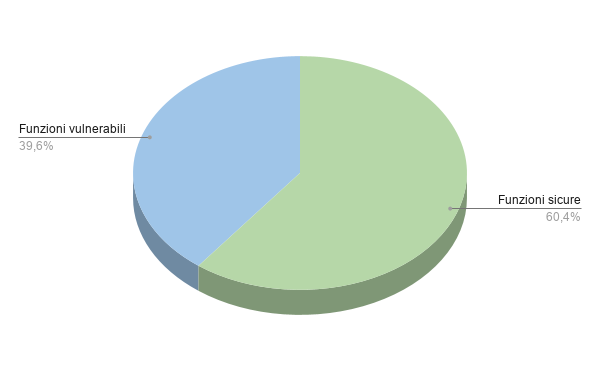
\includegraphics[width=0.60\textwidth]{immagini/Torta dataset.png}
    \caption{Suddivisione del dataset}
    \label{fig:Dataset_baseline}
\end{figure}

Poiché l'obiettivo della ricerca è valutare l'efficacia degli attacchi nell'indurre in errore i modelli e come questi ultimi operano, è metodologicamente necessario applicare tali perturbazioni esclusivamente agli snippet che il modello è originariamente in grado di classificare in modo corretto. Un attacco su un frammento di codice che il modello già sbaglia a classificare in condizioni normali risulterebbe privo di scopo.
Per tale motivo al termine dell'esecuzione della baseline sono stati creati dei dataset più piccoli a partire dal quello originale:

\begin{itemize}
    \item \texttt{df\_modello\_TP:} Rappresenta il sottoinsieme dei codici vulnerabili che sono stati correttamente identificati. È strutturato a livello di singolo modello: uno specifico frammento di codice sarà presente tante volte quanti sono i modelli che lo hanno classificato con successo.
    \item \texttt{df\_modello\_TN:} Dataset filtrato contenente unicamente i codici sicuri correttamente identificati. I dati sono salvati in modalità modello-snippet, pertanto come per il dataset \texttt{df\_modello\_TP} lo stesso codice sicuro è replicato per ogni modello che lo ha identificato correttamente.
    \item \texttt{df\_modello\_TRUE:} È il dataset nato dalla concatenazione di \texttt{df\_modello\_TP} e \texttt{df\_modello\_TN}. Rappresenta quindi la raccolta, per ogni modello, di tutti i codici vulnerabili e sicuri correttamente identificati.
\end{itemize}

